\section{Eletrização por atrito. Gerador de Graaff}

\frame{
	\frametitle{Processos de eletrização}
	\begin{block}{Definição}
		Considera-se um corpo eletrizado quando este tiver número diferente de prótons e elétrons, ou seja, quando não estiver neutro. O processo de retirar ou acrescentar elétrons a um corpo neutro para que este passa a estar eletrizado denomina-se \textbf{eletrização}.
	\end{block}
}

\frame{
	\frametitle{Processos de eletrização}
	\begin{block}{Contextualização}
		Em alguns momentos do nosso cotidiano, deparamo-nos com situações um “pouco estranhas”, nas quais tomamos choques em maçanetas de portas, na tela da TV ou até mesmo quando encostamos em outra pessoa. Esses pequenos choques ocorrem em razão da eletricidade estática que adquirimos diariamente.
	\end{block}
}

\frame{
	\frametitle{Processos de eletrização}
	\centerline{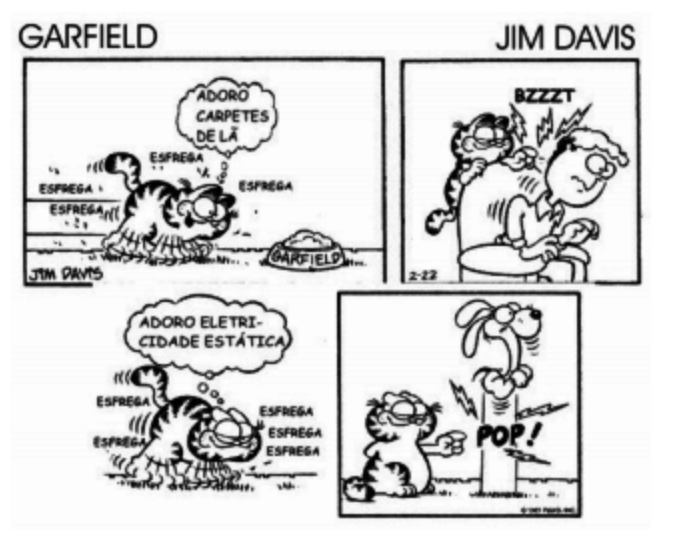
\includegraphics[width=0.8\linewidth]{Figuras/Ch03/estatica.PNG}}
}

\frame{
	\frametitle{Processos de eletrização}
	\begin{block}{Tipos}
		\begin{itemize}
			\item Eletrização por atrito
			\item Eletrização por contato
			\item Eletrização por indução
		\end{itemize}
	\end{block}
}

\frame{
	\frametitle{Eletrização por atrito}
	\begin{block}{Lembra de Tales de Mileto?}
		\begin{itemize}
			\item Descobre que ao se esfregar âmbar (resina vegetal fóssil petrificada) com pele de carneiro, observa-se que pedaços de palha e penas eram atraídos pelo âmbar.
		\end{itemize}
	\end{block}
	\centerline{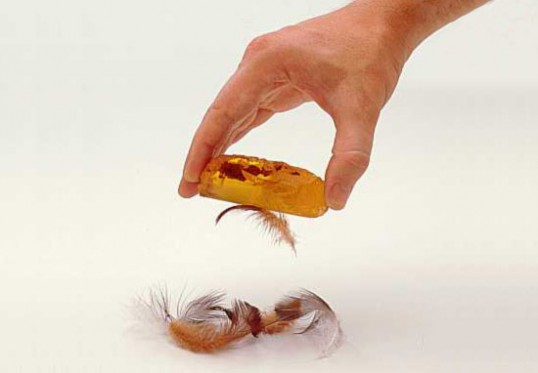
\includegraphics[width=0.6\linewidth]{Figuras/Ch01/ambar.JPG}}
}

\frame{
	\frametitle{Eletrização por atrito}
	\begin{block}{Avanço}
		Posteriormente o estudo de Tales foi expandido, sendo possível comprovar que \textbf{dois corpos neutros} feitos de materiais distintos, quando são atritados entre si, um deles fica eletrizado \textbf{negativamente} (ganha elétrons) e outro \textbf{positivamente} (perde elétrons).
	\end{block}
}

\frame{
	\frametitle{Eletrização por atrito}
	\begin{block}{Dependência do material}
		\begin{itemize}
			\item Quando há eletrização por atrito, os dois corpos ficam com cargas de módulo igual, porém com sinais opostos. Esta eletrização depende também da natureza do material, por exemplo, atritar um material $m_1$ com uma material $m_2$ pode deixar $m_1$  carregado negativamente e $m_2$ positivamente, enquanto o atrito entre o material $m_1$ e outro material $m_3$ é capaz de deixar $m_1$ carregado positivamente e $m_3$ negativamente.
			\item A eletrização por atrito é mais forte quando é feita por corpos isolantes, pois os elétrons permanecem nas regiões atritadas.
		\end{itemize}
	\end{block}
}

\frame{
	\frametitle{Eletrização por atrito}
	\begin{block}{Série triboelétrica}
		Lista em dada ordem que um elemento ao ser atritado com o sucessor da lista fica eletrizado positivamente.
	\end{block}
}

\frame{
	\frametitle{Eletrização por atrito}
	\begin{block}{Materiais}
		\begin{itemize}
			\item \tikzmark{p1}Pele humana seca
			\item Couro
			\item Pele de coelho
			\item Vidro
			\item Cabelo humano
			\item Fibra sintética
			\item Lã
			\item Chumbo
			\item Pele de gato
			\item Seda
			\item Alumínio
			\item \tikzmark{p2}Papel
		\end{itemize}
	\end{block}

	\begin{tikzpicture}[overlay, remember picture]
		\draw[-Latex,line width=2pt] ($ (p1)+(2,0) $) node[right] {$ + $} -- ($ (p2)+(2,0) $) node[right] {$ - $};
	\end{tikzpicture}
%	\centerline{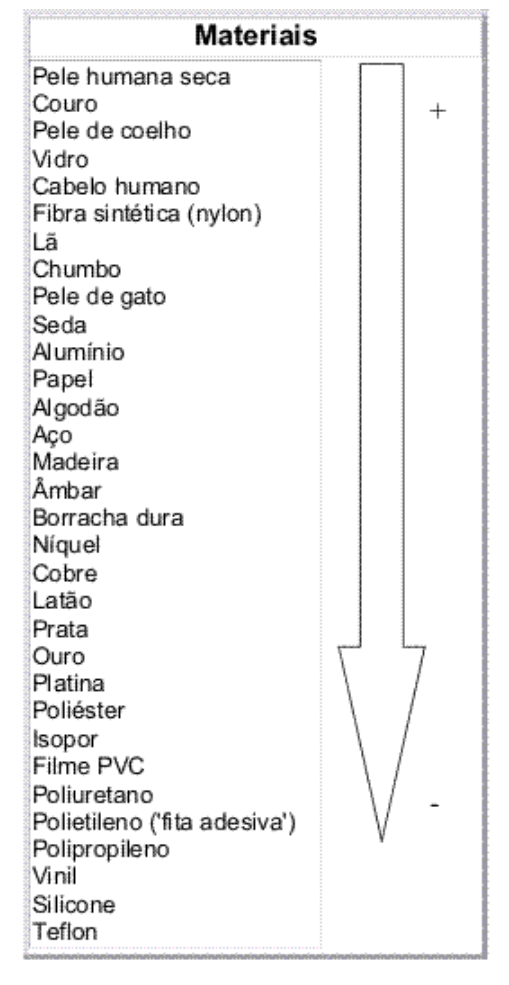
\includegraphics[width=0.35\linewidth]{Figuras/Ch03/serie.PNG}}
}

\frame{
	\frametitle{Eletrização por atrito}
	\begin{block}{Materiais}
		\begin{itemize}			
			\item \tikzmark{p1}Algodão
			\item Aço
			\item Madeira
			\item Âmbar
			\item Borracha dura
			\item Níquel
			\item Cobre
			\item Latão
			\item Prata
			\item Ouro
			\item Platina
			\item \tikzmark{p2}Poliéster
		\end{itemize}
	\end{block}
	
	\begin{tikzpicture}[overlay, remember picture]
	\draw[-Latex,line width=2pt] ($ (p1)+(2,0) $) node[right] {$ + $} -- ($ (p2)+(2,0) $) node[right] {$ - $};
	\end{tikzpicture}
	%	\centerline{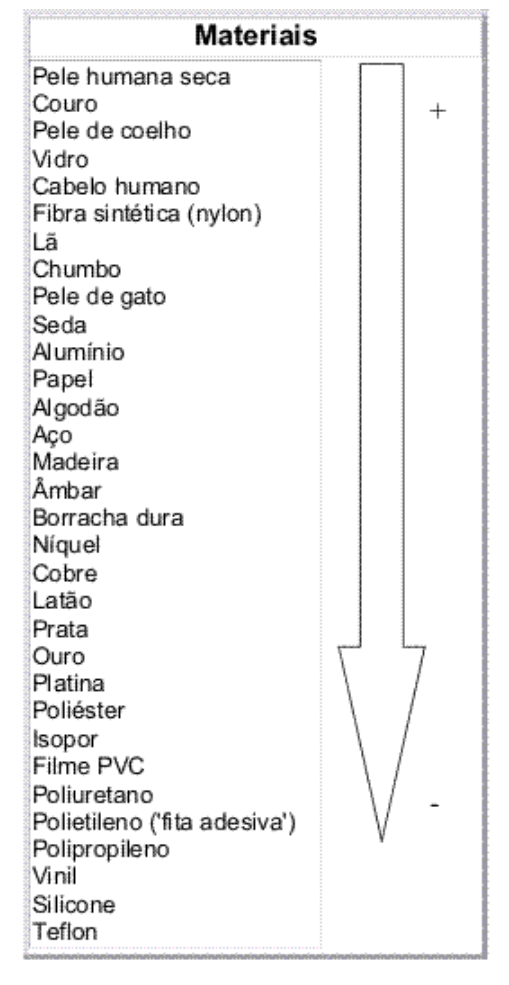
\includegraphics[width=0.35\linewidth]{Figuras/Ch03/serie.PNG}}
}

\frame{
	\frametitle{Eletrização por atrito}
	\begin{block}{Materiais}
		\begin{itemize}
			\item \tikzmark{p1}Isopor
			\item Filme PVC
			\item Poliuretano
			\item Polietileno (``fita adesiva'')
			\item Polipropileno
			\item Vinil
			\item Silicone
			\item \tikzmark{p2}Teflon
		\end{itemize}
	\end{block}
	
	\begin{tikzpicture}[overlay, remember picture]
	\draw[-Latex,line width=2pt] ($ (p1)+(2,0) $) node[right] {$ + $} -- ($ (p2)+(2,0) $) node[right] {$ - $};
	\end{tikzpicture}
	%	\centerline{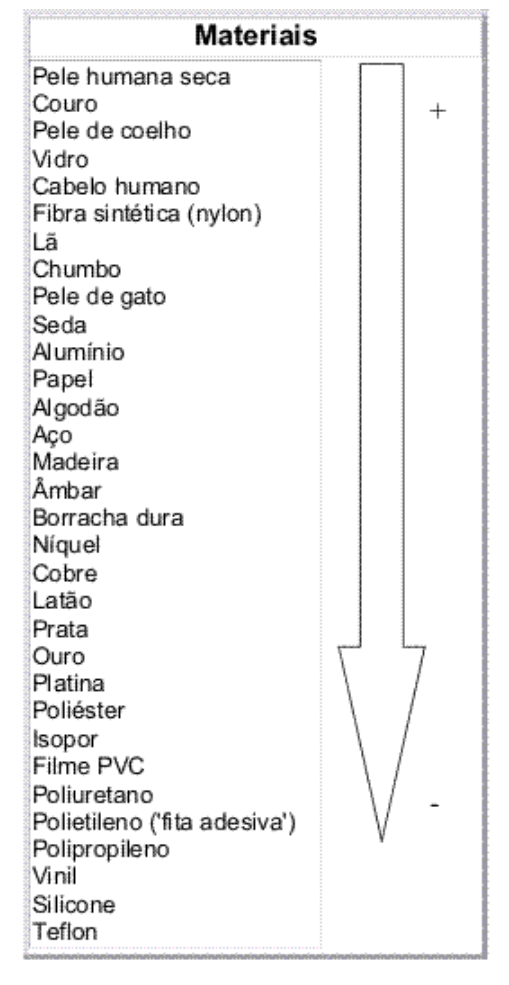
\includegraphics[width=0.35\linewidth]{Figuras/Ch03/serie.PNG}}
}

\frame{
	\frametitle{Eletrização por atrito}
	\begin{block}{Série triboelétrica}
		Se atritarmos, por exemplo, lã com isopor, a lã ficará carregada positivamente, enquanto que o isopor ficará carregado negativamente. Isso quer dizer, que durante o atrito, a lã perdeu elétrons e o isopor, por sua vez, ganhou elétrons.
	\end{block}
}

\frame{
	\frametitle{Eletrização por atrito}
	\begin{block}{Experiência}
		\begin{enumerate}
			\item Corte alguns pedaços de papel bem pequenos.
			\item Pegue uma caneta esferográfica.
			\item Atrite a parte de trás da caneta em seu cabelo.
			\item Aproxime a parte atritada aos pedaços de papel.
		\end{enumerate}
	\end{block}
	\centerline{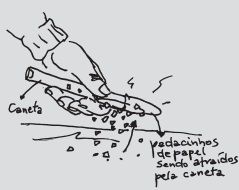
\includegraphics[width=0.45\linewidth]{Figuras/Ch03/caneta.jpg}}
}

\frame{
	\frametitle{Eletrização por atrito}
	\begin{block}{Experiência - por que isso acontece?}
		Isso ocorre porque quando você atritou a caneta no seu cabelo, houve uma transferência de elétrons entre os dois corpos, o que deixou a caneta carregada eletricamente. Ao aproximar essa caneta dos pedaços de papel, que são neutros, eles serão atraídos.
	\end{block}
}

\frame{
	\frametitle{Gerador de Van de Graaff}
	\begin{block}{Introdução}
		O chamado gerador de Van de Graaff foi idealizado pelo engenheiro americano Robert J. Van de Graaff, em 1929, com o objetivo de atingir altas tensões. Esse equipamento foi indispensável para condução das pesquisas sobre a constituição dos átomos e pesquisas nucleares.
	\end{block}
	\centerline{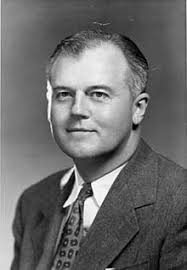
\includegraphics[width=0.25\linewidth]{Figuras/Ch03/van.jpg}}
}

\frame{
	\frametitle{Gerador de Van de Graaff}
	\begin{block}{O equipamento}
		Um motor movimenta uma correia isolante que passa por duas polias, uma delas acionada por um motor elétrico que faz a correia se movimentar. Através de pontas metálicas a correia recebe carga elétrica de um gerador de alta tensão. Esse movimento eletriza a correia por atrito, que sobe pelo lado esquerdo eletrizada. A segunda polia encontra-se dentro da esfera metálica oca. A correia eletrizada transporta as cargas até o interior da esfera metálica, onde elas são coletadas por pontas metálicas e conduzidas para a superfície externa da esfera.
	\end{block}
}

\frame{
	\frametitle{Gerador de Van de Graaff}
	\centerline{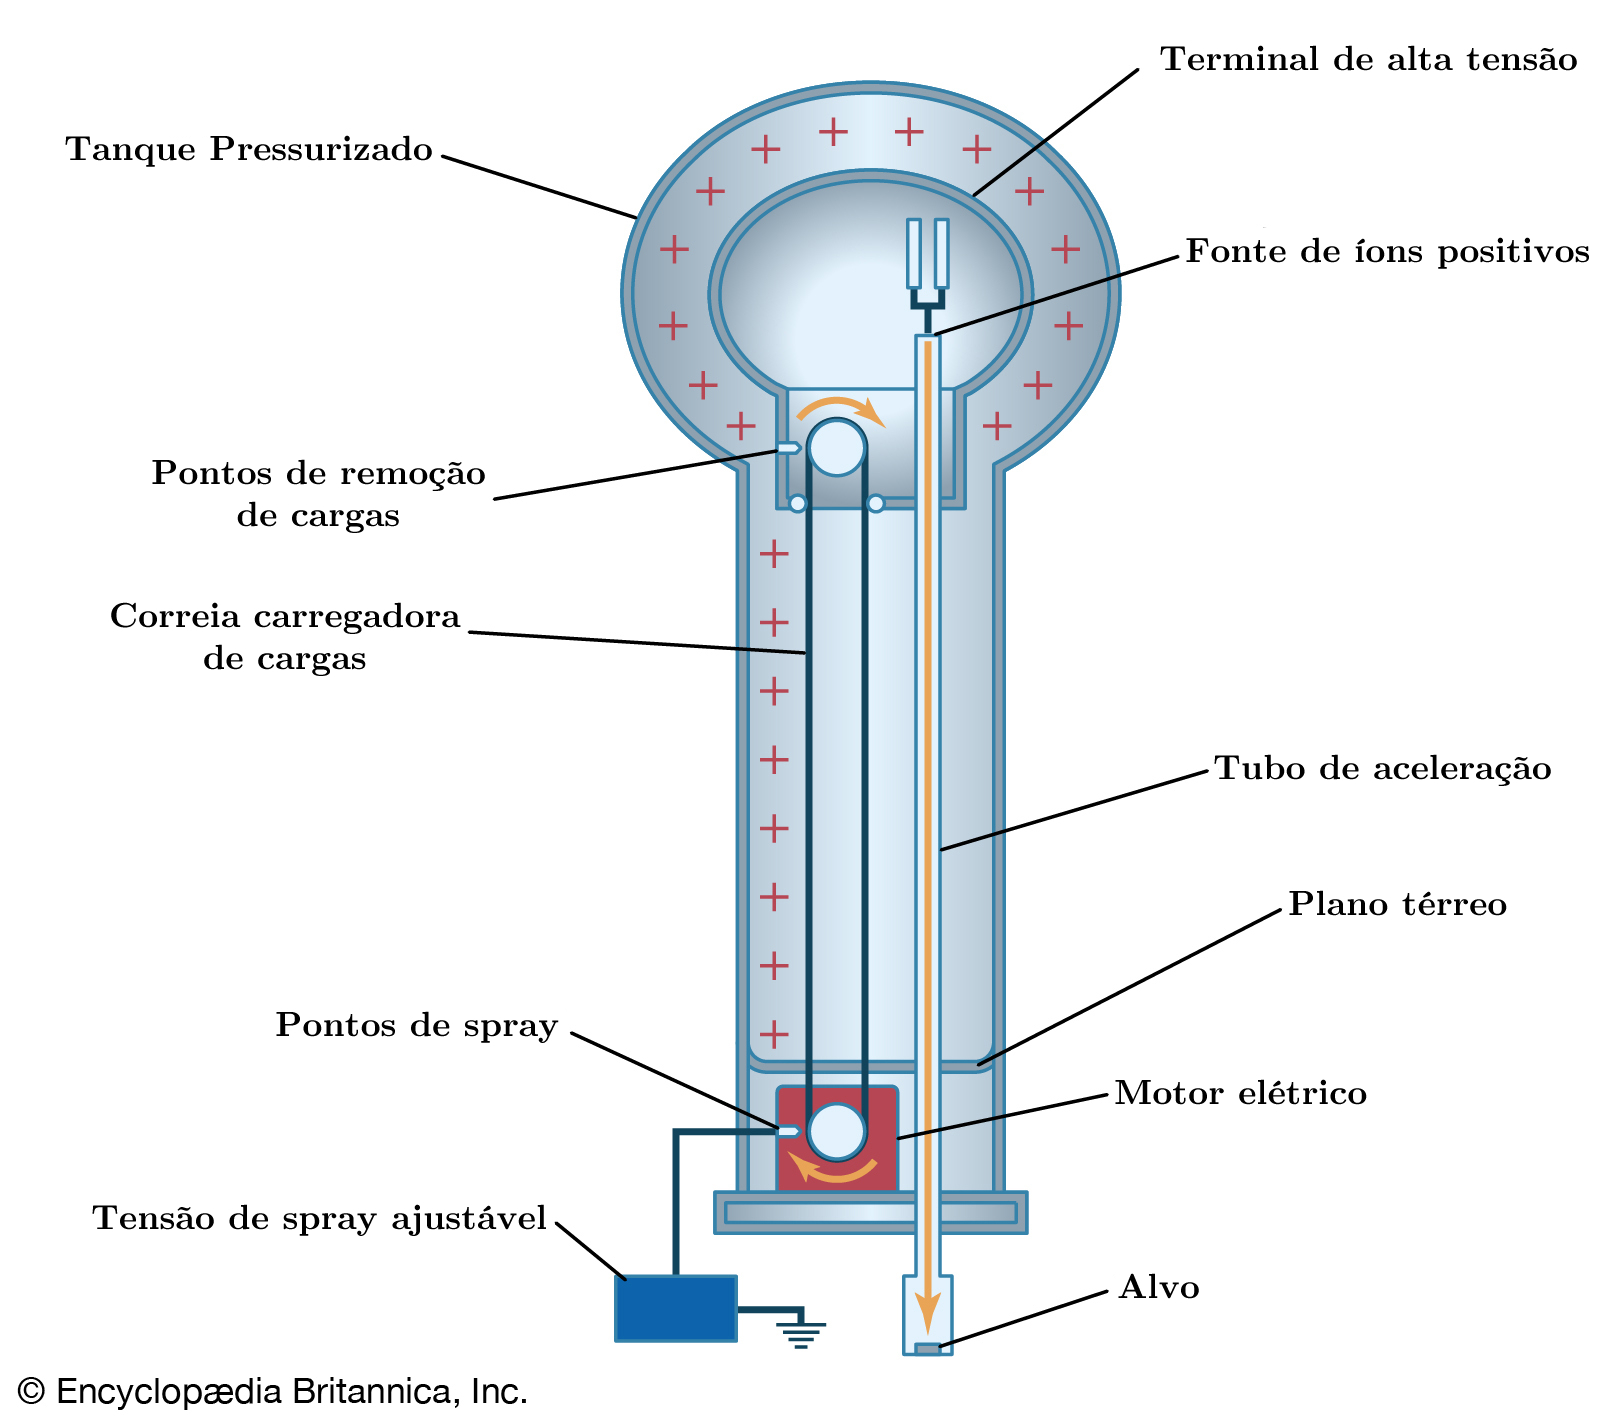
\includegraphics[height=0.9\textheight]{Figuras/Ch03/gerador12.jpg}}
}

\frame{
	\frametitle{Gerador de Van de Graaff}
	\centerline{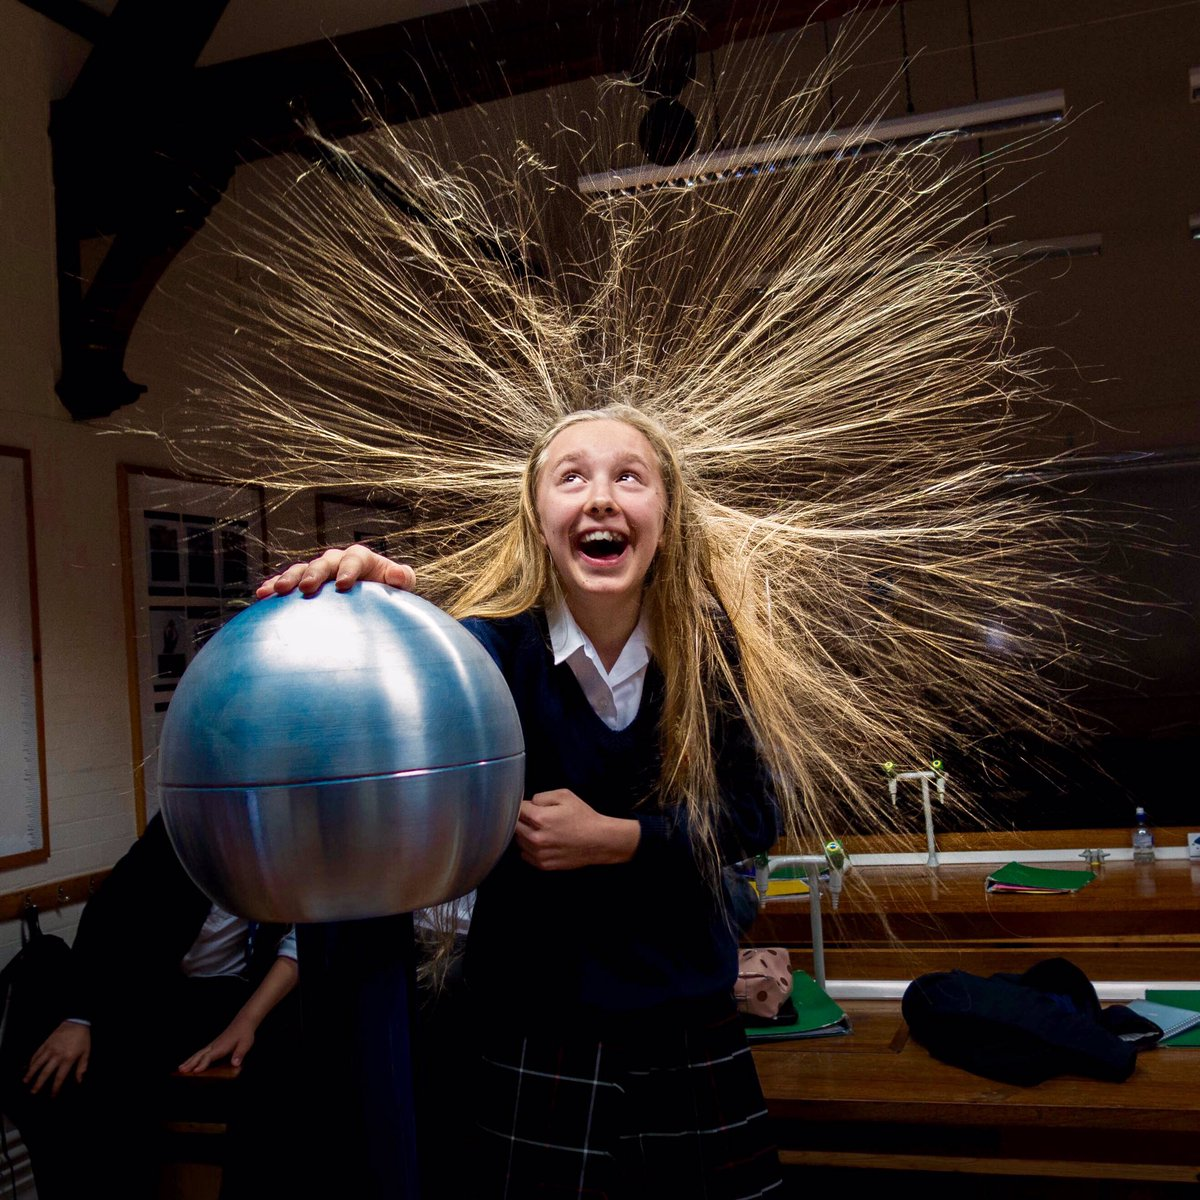
\includegraphics[width=0.6\linewidth]{Figuras/Ch03/gerador2.jpg}}
}

\frame{
	\frametitle{Gerador de Van de Graaff}
	\begin{block}{E o choque?}
		\begin{itemize}
			\item À medida que a esfera vai ficando carregada negativamente, parte deste excesso de cargas negativas vai passando gradativamente para o corpo da pessoa. Como ela está isolada do chão e o processo de eletrização é lento, ela não leva choque elétrico, mas vai recebendo cargas negativas e ficando carregada também. Desta forma todo o seu corpo se eletriza com carga do mesmo sinal das cargas da esfera, ou seja, negativas.
			\item Os fios de cabelos, leves e maleáveis, também vão ficando negativos. Com cargas de mesmo sinal, estes fios se repelem, afastando-se uns dos outros, provocando este efeito curioso e cabelo ouriçado!
		\end{itemize}
	\end{block}
}

\section*{Exercícios}

\frame{
	\frametitle{Exercícios}
	\begin{block}{}
		01. Um estudante atrita um pente de plástico em seu cabelo e aproxima-o de um filete de água, que imediatamente se encurva na direção do pente. Marque a alternativa que explica de forma correta o motivo pelo qual isso ocorre.

		\vspace{0.5cm}

		(a) O fenômeno é possível porque a água é um condutor universal.

		\vspace{0.3cm}

		(b) Após o atrito, o pente adquire a mesma carga elétrica da água, por isso, o filete é atraído.

		\vspace{0.3cm}

		(c) As cargas elétricas em excesso no pente atraem as cargas de mesmo sinal da água, fazendo com que o filete sofra deflexão.

		\vspace{0.3cm}

		(d) As cargas elétricas em excesso no pente atraem as cargas de sinal oposto da água, fazendo com que o filete sofra deflexão.

		\vspace{0.3cm}

		(e) Todas as alternativas estão incorretas.
	\end{block}
}

\section*{Referências}

\frame{
	\frametitle{Referências e Exercícios Complementares}
	\begin{itemize}
		\item Física, Ciência e Tecnologia – Vol 3. PENTEADO, Paulo César M; TORRES, Carlos Magno A. Ed. Moderna (2006)
	\end{itemize}
	%\centering{\alert{Página 36 - \textbf{1.6.1 até 1.6.5, 1.6.17 até 1.6.19}}} \\
	%https://www.youtube.com/watch?v=IUgS7Uw-qBI
	\centering{\alert{Lista de exercícios 03}}
}